\begin{figure}[t]
\centering
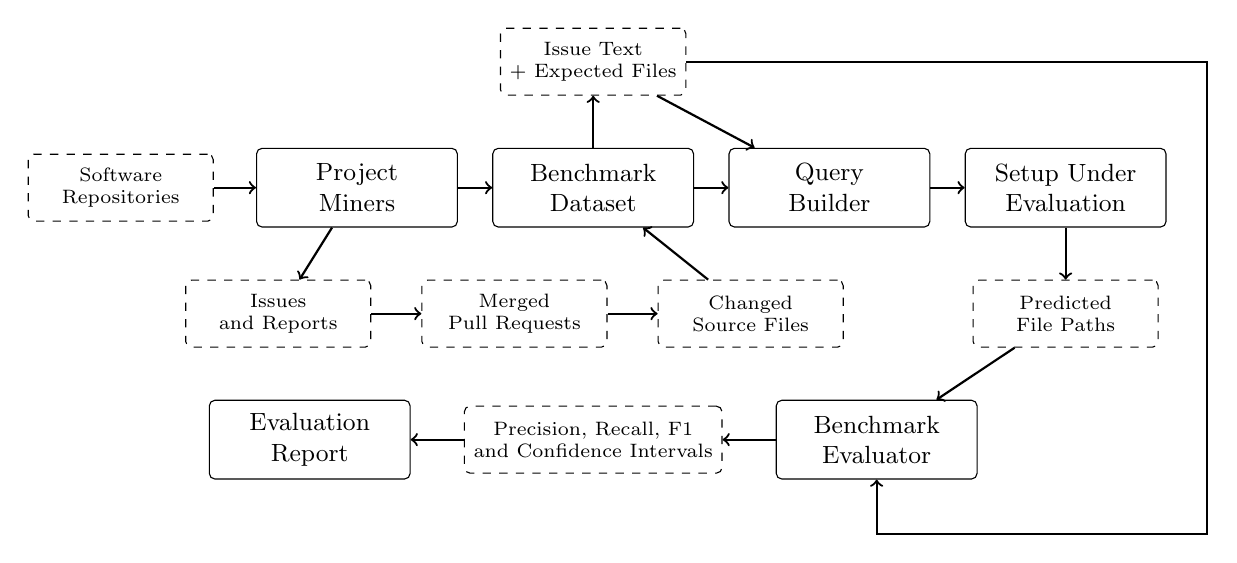
\begin{tikzpicture}[
  box/.style={
    draw,
    rectangle,
    rounded corners=2pt,
    align=center,
    minimum width=2.55cm,
    minimum height=1.0cm,
    font=\small
  },
  smallbox/.style={
    draw,
    rectangle,
    rounded corners=2pt,
    align=center,
    minimum width=2.35cm,
    minimum height=0.85cm,
    font=\scriptsize
  },
  databox/.style={
    draw,
    dashed,
    rectangle,
    rounded corners=2pt,
    align=center,
    minimum width=2.35cm,
    minimum height=0.85cm,
    font=\scriptsize
  },
  arrow/.style={->, thick}
]

% Input repositories and project mining.
\node[databox] (repos) at (0,2.5) {Software\\Repositories};
\node[box] (miner) at (3,2.5) {Project\\Miners};
\node[databox] (issues) at (2,0.9) {Issues\\and Reports};
\node[databox] (prs) at (5,0.9) {Merged\\Pull Requests};
\node[databox] (diffs) at (8,0.9) {Changed\\Source Files};

% Benchmark construction.
\node[box] (dataset) at (6,2.5) {Benchmark\\Dataset};
\node[databox] (instance) at (6,4.1) {Issue Text\\+ Expected Files};

% Querying setups under evaluation.
\node[box] (query) at (9,2.5) {Query\\Builder};
\node[box] (setups) at (12,2.5) {Setup Under\\Evaluation};
\node[databox] (predictions) at (12,0.9) {Predicted\\File Paths};

% Evaluation and reporting.
\node[box] (evaluator) at (9.6,-0.7) {Benchmark\\Evaluator};
\node[databox] (metrics) at (6,-0.7) {Precision, Recall, F1\\and Confidence Intervals};
\node[box] (report) at (2.4,-0.7) {Evaluation\\Report};

% Main workflow arrows.
\draw[arrow] (repos) -- (miner);
\draw[arrow] (miner) -- (dataset);
\draw[arrow] (dataset) -- (query);
\draw[arrow] (query) -- (setups);

% Mining details.
\draw[arrow] (miner) -- (issues);
\draw[arrow] (issues) -- (prs);
\draw[arrow] (prs) -- (diffs);
\draw[arrow] (diffs) -- (dataset);

% Benchmark instance and prediction loop.
\draw[arrow] (dataset) -- (instance);
\draw[arrow] (instance) -- (query);
\draw[arrow] (setups) -- (predictions);
\draw[arrow] (predictions) -- (evaluator);
\draw[arrow] (instance.east) -- (13.8,4.1) -- (13.8,-1.9) -- (9.6,-1.9) -- (evaluator.south);

% Evaluation outputs.
\draw[arrow] (evaluator) -- (metrics);
\draw[arrow] (metrics) -- (report);

\end{tikzpicture}
\caption{Generic workflow for constructing and evaluating a code localization benchmark. Project miners extract issue reports, merged code changes, and impacted files from software repositories. Each benchmark instance combines an issue description with ground-truth impacted source files. Setups under evaluation receive the issue-derived query and return predicted file paths, which are compared against the benchmark targets to compute evaluation metrics. Dashed boxes denote data artifacts, while solid boxes denote processes.}
\label{fig:benchmark-workflow}
\end{figure}
